\chapter{THIẾT KẾ MỨC VẬT LÍ}
\label{chap:trien_khai_csdl}

\section{XÁC ĐỊNH HỆ QUẢN TRỊ CƠ SỞ DỮ LIỆU}
Nhóm lựa chọn Microsoft SQL Server (Express/Developer Edition) làm hệ quản trị cơ sở dữ liệu (DBMS) để triển khai hệ thống AR\_IMMS dựa trên các lý do kỹ thuật và thực tiễn sau:

\begin{itemize}
    \item \textbf{Chi phí và Quy mô:} Miễn phí bản quyền sử dụng, hoàn toàn đủ khả năng đáp ứng quy mô đồ án với 16 thực thể dữ liệu.
    \item \textbf{Ràng buộc toàn vẹn:} Hỗ trợ đầy đủ và chặt chẽ các ràng buộc toàn vẹn dữ liệu như PRIMARY KEY, FOREIGN KEY, NOT NULL, UNIQUE, DEFAULT, và CHECK.
    \item \textbf{Công cụ quản lý:} Hỗ trợ công cụ quản lý trực quan SQL Server Management Studio (SSMS) giúp dễ dàng trong việc thiết kế, khởi tạo, viết truy vấn và kiểm thử dữ liệu.
    \item \textbf{Kiểu dữ liệu phù hợp:} Hỗ trợ tốt kiểu dữ liệu ngày giờ (DATETIME), đặc biệt phù hợp với nhóm dữ liệu TELEMETRY (dữ liệu chuỗi thời gian - time-series data).
    \item \textbf{Khả năng mở rộng:} Ngôn ngữ T-SQL mạnh mẽ, hỗ trợ tốt các thao tác nâng cao như JOIN, VIEW, STORED PROCEDURE, và TRIGGER nhằm phục vụ cho việc phát triển và mở rộng các nghiệp vụ phức tạp sau này.
\end{itemize}

\section{TẠO DATABASE AR\_IMMS}
Để triển khai hệ thống quản lý cơ sở dữ liệu AR-IMMS, nhóm sử dụng SQL Server làm hệ quản trị cơ sở dữ liệu. Cơ sở dữ liệu AR\_IMMS được khởi tạo nhằm lưu trữ và quản lý toàn bộ dữ liệu phục vụ cho hoạt động vận hành của hệ thống.

Database được khởi tạo bằng câu lệnh T-SQL sau:

\begin{lstlisting}[language=SQL]
CREATE DATABASE AR_IMMS;
GO
\end{lstlisting}

Hình ảnh minh họa việc khởi tạo Database trong SQL Server Management Studio (SSMS):

\begin{figure}[H]
    \centering
    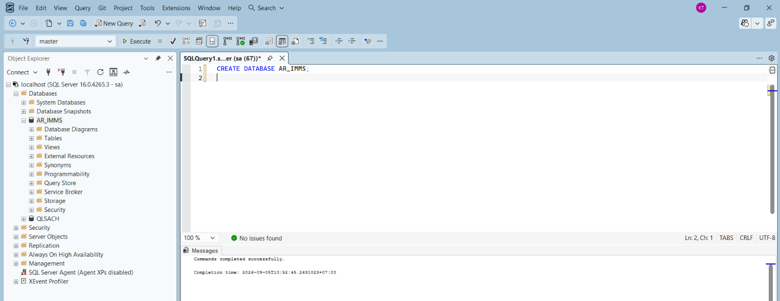
\includegraphics[width=0.95\textwidth]{imagesssms_create_db.png} % Thay duong dan anh cua ban
    \caption{Khởi tạo Database AR\_IMMS trong SSMS}
    \label{fig:create_db}
\end{figure}

\section{VIẾT LỆNH TẠO BẢNG}
\noindent \textbf{Hệ quản trị cơ sở dữ liệu:} SQL Server

\begin{lstlisting}[language=SQL]
-- 1. Bang ROLE
CREATE TABLE [ROLE] (
    role_id INT IDENTITY(1,1) PRIMARY KEY,
    role_name NVARCHAR(100) NOT NULL,
    description NVARCHAR(255) NULL
);

-- 2. Bang USER
CREATE TABLE [USER] (
    user_id INT IDENTITY(1,1) PRIMARY KEY,
    username VARCHAR(50) NOT NULL,
    password_hash VARCHAR(255) NOT NULL,
    full_name NVARCHAR(100) NOT NULL,
    email VARCHAR(100) NOT NULL,
    status VARCHAR(20) NOT NULL
);

-- 3. Bang USER_ROLE
CREATE TABLE [USER_ROLE] (
    user_role_id INT IDENTITY(1,1) PRIMARY KEY,
    user_id_fk INT NOT NULL,
    role_id_fk INT NOT NULL
);

-- 4. Bang SITE
CREATE TABLE [SITE] (
    site_id INT IDENTITY(1,1) PRIMARY KEY,
    site_name NVARCHAR(100) NOT NULL,
    location NVARCHAR(255) NOT NULL
);

-- 5. Bang ROOM
CREATE TABLE [ROOM] (
    room_id INT IDENTITY(1,1) PRIMARY KEY,
    room_name NVARCHAR(100) NOT NULL,
    site_id_fk INT NOT NULL
);

-- 6. Bang RACK
CREATE TABLE [RACK] (
    rack_id INT IDENTITY(1,1) PRIMARY KEY,
    rack_name NVARCHAR(100) NOT NULL,
    room_id_fk INT NOT NULL
);

-- 7. Bang SERVER
CREATE TABLE [SERVER] (
    server_id INT IDENTITY(1,1) PRIMARY KEY,
    server_name NVARCHAR(100) NOT NULL,
    ip_address VARCHAR(15) NOT NULL,
    operating_system NVARCHAR(100) NOT NULL,
    status VARCHAR(20) NOT NULL,
    rack_id_fk INT NOT NULL
);

-- 8. Bang CONTAINER
CREATE TABLE [CONTAINER] (
    container_id INT IDENTITY(1,1) PRIMARY KEY,
    container_name NVARCHAR(100) NOT NULL,
    container_type NVARCHAR(50) NULL,
    status VARCHAR(20) NOT NULL,
    server_id_fk INT NOT NULL
);

-- 9. Bang WARRANTY
CREATE TABLE [WARRANTY] (
    warranty_id INT IDENTITY(1,1) PRIMARY KEY,
    provider NVARCHAR(100) NOT NULL,
    warranty_start DATE NOT NULL,
    warranty_end DATE NOT NULL,
    status NVARCHAR(50) NOT NULL,
    server_id_fk INT NOT NULL
);

-- 10. Bang TELEMETRY
CREATE TABLE [TELEMETRY] (
    telemetry_id INT IDENTITY(1,1) PRIMARY KEY,
    cpu_usage FLOAT NOT NULL,
    ram_usage FLOAT NOT NULL,
    disk_usage FLOAT NOT NULL,
    network_usage FLOAT NULL,
    temperature FLOAT NULL,
    recorded_at DATETIME NOT NULL,
    server_id_fk INT NOT NULL
);

-- 11. Bang ALERT_THRESHOLD
CREATE TABLE [ALERT_THRESHOLD] (
    threshold_id INT IDENTITY(1,1) PRIMARY KEY,
    metric_name VARCHAR(50) NOT NULL,
    warning_value FLOAT NOT NULL,
    critical_value FLOAT NOT NULL,
    is_active BIT NOT NULL,
    server_id_fk INT NOT NULL
);

-- 12. Bang ALERT
CREATE TABLE [ALERT] (
    alert_id INT IDENTITY(1,1) PRIMARY KEY,
    alert_type VARCHAR(50) NOT NULL,
    severity VARCHAR(20) NOT NULL,
    description NVARCHAR(MAX) NULL,
    status VARCHAR(20) NOT NULL,
    created_at DATETIME NOT NULL,
    server_id_fk INT NOT NULL
);

-- 13. Bang INCIDENT
CREATE TABLE [INCIDENT] (
    incident_id INT IDENTITY(1,1) PRIMARY KEY,
    incident_title NVARCHAR(200) NOT NULL,
    description NVARCHAR(MAX) NULL,
    priority VARCHAR(20) NOT NULL,
    status VARCHAR(20) NOT NULL,
    created_at DATETIME NOT NULL,
    alert_id_fk INT NOT NULL
);

-- 14. Bang TICKET
CREATE TABLE [TICKET] (
    ticket_id INT IDENTITY(1,1) PRIMARY KEY,
    ticket_title NVARCHAR(200) NOT NULL,
    description NVARCHAR(MAX) NULL,
    priority VARCHAR(20) NOT NULL,
    status VARCHAR(20) NOT NULL,
    created_at DATETIME NOT NULL,
    incident_id_fk INT NOT NULL,
    assigned_user_id_fk INT NOT NULL
);

-- 15. Bang MAINTENANCE
CREATE TABLE [MAINTENANCE] (
    maintenance_id INT IDENTITY(1,1) PRIMARY KEY,
    maintenance_type NVARCHAR(100) NOT NULL,
    description NVARCHAR(MAX) NULL,
    performed_at DATETIME NOT NULL,
    result NVARCHAR(MAX) NULL,
    ticket_id_fk INT NOT NULL
);

-- 16. Bang AUDIT_LOG
CREATE TABLE [AUDIT_LOG] (
    audit_log_id INT IDENTITY(1,1) PRIMARY KEY,
    action NVARCHAR(200) NOT NULL,
    entity_type VARCHAR(50) NOT NULL,
    entity_id INT NULL,
    description NVARCHAR(MAX) NULL,
    created_at DATETIME NOT NULL,
    user_id_fk INT NULL
);
\end{lstlisting}

\section{THIẾT LẬP CONSTRAINT}
\noindent \textbf{Hệ quản trị:} SQL Server

\subsection{FOREIGN KEY}
\begin{lstlisting}[language=SQL]
USE AR_IMMS;
GO

-- USER_ROLE
ALTER TABLE [USER_ROLE]
ADD CONSTRAINT FK_USER_ROLE_USER
FOREIGN KEY (user_id_fk) REFERENCES [USER](user_id);

ALTER TABLE [USER_ROLE]
ADD CONSTRAINT FK_USER_ROLE_ROLE
FOREIGN KEY (role_id_fk) REFERENCES [ROLE](role_id);

-- ROOM
ALTER TABLE [ROOM]
ADD CONSTRAINT FK_ROOM_SITE
FOREIGN KEY (site_id_fk) REFERENCES [SITE](site_id);

-- RACK
ALTER TABLE [RACK]
ADD CONSTRAINT FK_RACK_ROOM
FOREIGN KEY (room_id_fk) REFERENCES [ROOM](room_id);

-- SERVER
ALTER TABLE [SERVER]
ADD CONSTRAINT FK_SERVER_RACK
FOREIGN KEY (rack_id_fk) REFERENCES [RACK](rack_id);

-- CONTAINER
ALTER TABLE [CONTAINER]
ADD CONSTRAINT FK_CONTAINER_SERVER
FOREIGN KEY (server_id_fk) REFERENCES [SERVER](server_id);

-- WARRANTY
ALTER TABLE [WARRANTY]
ADD CONSTRAINT FK_WARRANTY_SERVER
FOREIGN KEY (server_id_fk) REFERENCES [SERVER](server_id);

-- TELEMETRY (Da sua tham chieu thanh server_id)
ALTER TABLE [TELEMETRY]
ADD CONSTRAINT FK_TELEMETRY_SERVER
FOREIGN KEY (server_id_fk) REFERENCES [SERVER](server_id);

-- ALERT_THRESHOLD (Da sua tham chieu thanh server_id)
ALTER TABLE [ALERT_THRESHOLD]
ADD CONSTRAINT FK_ALERT_THRESHOLD_SERVER
FOREIGN KEY (server_id_fk) REFERENCES [SERVER](server_id);

-- ALERT (Da sua tham chieu thanh server_id)
ALTER TABLE [ALERT]
ADD CONSTRAINT FK_ALERT_SERVER
FOREIGN KEY (server_id_fk) REFERENCES [SERVER](server_id);

-- INCIDENT
ALTER TABLE [INCIDENT]
ADD CONSTRAINT FK_INCIDENT_ALERT
FOREIGN KEY (alert_id_fk) REFERENCES [ALERT](alert_id);

-- TICKET
ALTER TABLE [TICKET]
ADD CONSTRAINT FK_TICKET_INCIDENT
FOREIGN KEY (incident_id_fk) REFERENCES [INCIDENT](incident_id);

ALTER TABLE [TICKET]
ADD CONSTRAINT FK_TICKET_ASSIGNED_USER
FOREIGN KEY (assigned_user_id_fk) REFERENCES [USER](user_id);

-- MAINTENANCE
ALTER TABLE [MAINTENANCE]
ADD CONSTRAINT FK_MAINTENANCE_TICKET
FOREIGN KEY (ticket_id_fk) REFERENCES [TICKET](ticket_id);

-- AUDIT_LOG
ALTER TABLE [AUDIT_LOG]
ADD CONSTRAINT FK_AUDIT_LOG_USER
FOREIGN KEY (user_id_fk) REFERENCES [USER](user_id);
GO
\end{lstlisting}

\subsection{UNIQUE CONSTRAINT}
\begin{lstlisting}[language=SQL]
USE AR_IMMS;
GO

ALTER TABLE [ROLE]
ADD CONSTRAINT UQ_ROLE_NAME UNIQUE (role_name);

ALTER TABLE [USER]
ADD CONSTRAINT UQ_USER_USERNAME UNIQUE (username);

ALTER TABLE [USER]
ADD CONSTRAINT UQ_USER_EMAIL UNIQUE (email);

ALTER TABLE [USER_ROLE]
ADD CONSTRAINT UQ_USER_ROLE UNIQUE (user_id_fk, role_id_fk);

ALTER TABLE [SITE]
ADD CONSTRAINT UQ_SITE_NAME UNIQUE (site_name);

-- SERVER (Bo sung UNIQUE cho server_name va ip_address)
ALTER TABLE [SERVER]
ADD CONSTRAINT UQ_SERVER_NAME UNIQUE (server_name);

ALTER TABLE [SERVER]
ADD CONSTRAINT UQ_SERVER_IP UNIQUE (ip_address);

-- WARRANTY
ALTER TABLE [WARRANTY]
ADD CONSTRAINT UQ_WARRANTY_SERVER UNIQUE (server_id_fk);

-- ALERT_THRESHOLD
ALTER TABLE [ALERT_THRESHOLD]
ADD CONSTRAINT UQ_ALERT_THRESHOLD UNIQUE (server_id_fk, metric_name);
GO
\end{lstlisting}

\subsection{CHECK CONSTRAINT}
\begin{lstlisting}[language=SQL]
USE AR_IMMS;
GO

-- USER
ALTER TABLE [USER]
ADD CONSTRAINT CK_USER_STATUS
CHECK (status IN ('ACTIVE', 'INACTIVE'));

-- SERVER
ALTER TABLE [SERVER]
ADD CONSTRAINT CK_SERVER_STATUS
CHECK (status IN ('ONLINE', 'OFFLINE', 'MAINTENANCE', 'INACTIVE'));

-- CONTAINER
ALTER TABLE [CONTAINER]
ADD CONSTRAINT CK_CONTAINER_STATUS
CHECK (status IN ('RUNNING', 'STOPPED', 'PAUSED', 'INACTIVE'));

-- WARRANTY
ALTER TABLE [WARRANTY]
ADD CONSTRAINT CK_WARRANTY_DATE
CHECK (warranty_end >= warranty_start);

-- TELEMETRY
ALTER TABLE [TELEMETRY]
ADD CONSTRAINT CK_TELEMETRY_CPU
CHECK (cpu_usage >= 0 AND cpu_usage <= 100);

ALTER TABLE [TELEMETRY]
ADD CONSTRAINT CK_TELEMETRY_RAM
CHECK (ram_usage >= 0 AND ram_usage <= 100);

ALTER TABLE [TELEMETRY]
ADD CONSTRAINT CK_TELEMETRY_DISK
CHECK (disk_usage >= 0 AND disk_usage <= 100);

-- ALERT_THRESHOLD
ALTER TABLE [ALERT_THRESHOLD]
ADD CONSTRAINT CK_THRESHOLD_VALUES
CHECK (warning_value >= 0 AND critical_value >= warning_value);

-- ALERT
ALTER TABLE [ALERT]
ADD CONSTRAINT CK_ALERT_SEVERITY
CHECK (severity IN ('WARNING', 'CRITICAL'));

ALTER TABLE [ALERT]
ADD CONSTRAINT CK_ALERT_STATUS
CHECK (status IN ('OPEN', 'ACKNOWLEDGED', 'RESOLVED', 'CLOSED'));

-- INCIDENT
ALTER TABLE [INCIDENT]
ADD CONSTRAINT CK_INCIDENT_PRIORITY
CHECK (priority IN ('LOW', 'MEDIUM', 'HIGH', 'CRITICAL'));

ALTER TABLE [INCIDENT]
ADD CONSTRAINT CK_INCIDENT_STATUS
CHECK (status IN ('OPEN', 'IN_PROGRESS', 'RESOLVED', 'CLOSED'));

-- TICKET
ALTER TABLE [TICKET]
ADD CONSTRAINT CK_TICKET_PRIORITY
CHECK (priority IN ('LOW', 'MEDIUM', 'HIGH', 'CRITICAL'));

ALTER TABLE [TICKET]
ADD CONSTRAINT CK_TICKET_STATUS
CHECK (status IN ('OPEN', 'IN_PROGRESS', 'RESOLVED', 'CLOSED'));
GO
\end{lstlisting}

\subsection{DEFAULT CONSTRAINT}
\begin{lstlisting}[language=SQL]
USE AR_IMMS;
GO

ALTER TABLE [USER]
ADD CONSTRAINT DF_USER_STATUS DEFAULT 'Inactive' FOR status;

ALTER TABLE [SERVER]
ADD CONSTRAINT DF_SERVER_STATUS DEFAULT 'Inactive' FOR status;

ALTER TABLE [CONTAINER]
ADD CONSTRAINT DF_CONTAINER_STATUS DEFAULT 'Inactive' FOR status;

ALTER TABLE [ALERT_THRESHOLD]
ADD CONSTRAINT DF_ALERT_THRESHOLD_ACTIVE DEFAULT 1 FOR is_active;

ALTER TABLE [ALERT]
ADD CONSTRAINT DF_ALERT_STATUS DEFAULT 'OPEN' FOR status;

ALTER TABLE [ALERT]
ADD CONSTRAINT DF_ALERT_CREATED_AT DEFAULT GETDATE() FOR created_at;

ALTER TABLE [INCIDENT]
ADD CONSTRAINT DF_INCIDENT_STATUS DEFAULT 'OPEN' FOR status;

ALTER TABLE [INCIDENT]
ADD CONSTRAINT DF_INCIDENT_CREATED_AT DEFAULT GETDATE() FOR created_at;

ALTER TABLE [TICKET]
ADD CONSTRAINT DF_TICKET_STATUS DEFAULT 'OPEN' FOR status;

ALTER TABLE [TICKET]
ADD CONSTRAINT DF_TICKET_CREATED_AT DEFAULT GETDATE() FOR created_at;

ALTER TABLE [MAINTENANCE]
ADD CONSTRAINT DF_MAINTENANCE_PERFORMED_AT DEFAULT GETDATE() FOR performed_at;

ALTER TABLE [AUDIT_LOG]
ADD CONSTRAINT DF_AUDIT_LOG_CREATED_AT DEFAULT GETDATE() FOR created_at;
GO
\end{lstlisting}

\section{CHÈN DỮ LIỆU}
Dữ liệu mẫu của nhóm được sử dụng để kiểm thử cơ sở dữ liệu được tạo bằng công cụ Mockaroo. Dữ liệu được xây dựng dựa trên cấu trúc 16 bảng, các thuộc tính và mối quan hệ đã thiết kế ở các chương trước. Sau khi tạo, dữ liệu được kiểm tra và điều chỉnh để đảm bảo tính hợp lệ của các khóa chính, khóa ngoại và các ràng buộc trong cơ sở dữ liệu. 

\vspace{0.5em}
\noindent \textbf{THỨ TỰ NHẬP DỮ LIỆU CHO DATABASE AR\_IMMS}

\subsection{QUẢN LÝ NGƯỜI DÙNG \& PHÂN QUYỀN (USER -- ROLE -- USER\_ROLE)}

\paragraph{a. Bảng ROLE (Vai trò / Nhóm quyền)}
\begin{itemize}
    \item \textbf{Mục đích:} Khởi tạo danh mục nhóm quyền (Admin, Operator, Technician).
    \item \textbf{Lý do nạp trước:} Là bảng danh mục chuẩn hóa độc lập, không phụ thuộc vào các bảng khác.
\end{itemize}

\paragraph{b. Bảng USER (Tài khoản người dùng)}
\begin{itemize}
    \item \textbf{Mục đích:} Lưu thông tin cá nhân và tài khoản đăng nhập của nhân viên.
    \item \textbf{Lý do nạp trước USER\_ROLE:} Cần tạo danh sách tài khoản người dùng trước để có \texttt{user\_id} tham chiếu.
\end{itemize}

\paragraph{c. Bảng USER\_ROLE (Phân quyền tài khoản)}
\begin{itemize}
    \item \textbf{Mục đích:} Gán vai trò/quyền hạn cụ thể cho từng tài khoản.
    \item \textbf{Lý do nạp cuối Phần 2:} Bảng này đóng vai trò giải quyết mối quan hệ Nhiều - Nhiều (N-N), bắt buộc phải có sẵn cả \texttt{user\_id\_fk} và \texttt{role\_id\_fk} từ hai bảng trên mới có thể thực hiện liên kết.
\end{itemize}

\subsection{HẠ TẦNG VẬT LÝ \& THU THẬP DỮ LIỆU (SITE -- ROOM -- RACK -- SERVER -- TELEMETRY)}

\paragraph{a. Bảng SITE (Trung tâm dữ liệu)}
\begin{itemize}
    \item \textbf{Mục đích:} Lưu thông tin các vị trí trung tâm dữ liệu vật lý (Hà Nội, TP.HCM, Đà Nẵng).
    \item \textbf{Lý do nạp trước:} Đây là thực thể gốc cấp cao nhất trong hệ thống hạ tầng, độc lập và không chứa bất kỳ khóa ngoại (FK) nào.
\end{itemize}

\paragraph{b. Bảng ROOM (Phòng máy chủ)}
\begin{itemize}
    \item \textbf{Mục đích:} Lưu trữ danh sách các phòng máy chủ thuộc từng trung tâm dữ liệu.
    \item \textbf{Lý do nạp sau SITE:} Mỗi phòng máy bắt buộc phải thuộc một Site xác định thông qua \texttt{site\_id\_fk}. Cần có dữ liệu SITE trước để lấy ID tham chiếu hợp lệ.
\end{itemize}

\paragraph{c. Bảng RACK (Tủ Rack)}
\begin{itemize}
    \item \textbf{Mục đích:} Quản lý vị trí các tủ đĩa/tủ chứa thiết bị trong phòng máy.
    \item \textbf{Lý do nạp sau ROOM:} Mỗi tủ Rack phải được định vị bên trong một phòng máy cụ thể thông qua \texttt{room\_id\_fk}.
\end{itemize}

\paragraph{d. Bảng SERVER (Máy chủ vật lý)}
\noindent Ở bảng SERVER sẽ đc lấy dữ liệu từ file csv (\url{https://drive.google.com/file/d/1gjNlxpAloXAcxYxCO2b5VRABCf3k2lhI/view?usp=sharing})
\begin{itemize}
    \item \textbf{Mục đích:} Định danh máy chủ, lưu thông tin cấu hình phần cứng và vị trí lắp đặt.
    \item \textbf{Lý do nạp sau RACK:} Máy chủ vật lý phải được gán cố định vào một tủ Rack xác định thông qua \texttt{rack\_id\_fk}.
\end{itemize}

\paragraph{e. Bảng TELEMETRY (Dữ liệu giám sát cảm biến)}
\noindent Ở bảng TELEMETRY sẽ đc lấy dữ liệu từ file csv (\url{https://drive.google.com/file/d/1gjNlxpAloXAcxYxCO2b5VRABCf3k2lhI/view?usp=sharing})
\begin{itemize}
    \item \textbf{Mục đích:} Lưu các chỉ số vận hành thu thập theo thời gian thực (CPU, RAM, Nhiệt độ).
    \item \textbf{Lý do nạp sau SERVER:} Dữ liệu cảm biến không thể tồn tại độc lập mà bắt buộc phải gắn với một máy chủ cụ thể thông qua \texttt{server\_id\_fk}.
\end{itemize}

\subsection{Môi trường ảo và thông tin bảo hành (CONTAINER -- WARRANTY)}

\paragraph{a. Bảng CONTAINER (Môi trường ảo hóa)}
\begin{itemize}
    \item \textbf{Mục đích:} Quản lý các Container/Microservices đang chạy trên nền tảng máy chủ.
    \item \textbf{Lý do nạp sau SERVER:} Mọi môi trường ảo hóa đều phải được triển khai và cấp phát tài nguyên trên một máy chủ vật lý xác định (\texttt{server\_id\_fk}).
\end{itemize}

\paragraph{b. Bảng WARRANTY (Thông tin bảo hành)}
\begin{itemize}
    \item \textbf{Mục đích:} Quản lý thời hạn và hợp đồng bảo hành của thiết bị.
    \item \textbf{Lý do nạp sau SERVER:} Hợp đồng bảo hành được ký kết và áp dụng trực tiếp cho từng đầu máy chủ cụ thể (\texttt{server\_id\_fk}).
\end{itemize}

\subsection{VẬN HÀNH, GIÁM SÁT \& TRUY VẾT (ALERT\_THRESHOLD -- ALERT -- INCIDENT -- TICKET -- MAINTENANCE -- AUDIT\_LOG)}

\paragraph{a. Bảng ALERT\_THRESHOLD (Cấu hình ngưỡng)}
\begin{itemize}
    \item \textbf{Mục đích:} Cài đặt giới hạn cảnh báo (Warning/Critical) cho các chỉ số phần cứng của từng Server.
    \item \textbf{Lý do nạp trước ALERT:} Phải định nghĩa quy chuẩn ngưỡng an toàn trước làm cơ sở so sánh dữ liệu.
\end{itemize}

\paragraph{b. Bảng ALERT (Cảnh báo hệ thống)}
\begin{itemize}
    \item \textbf{Mục đích:} Lưu các thông báo cảnh báo phát sinh khi hạ tầng gặp bất thường.
    \item \textbf{Lý do nạp sau TELEMETRY \& ALERT\_THRESHOLD:} Dữ liệu trong ALERT được sinh ra bằng cách quét chỉ số từ TELEMETRY và so sánh với giá trị định sẵn trong ALERT\_THRESHOLD.
\end{itemize}

\paragraph{c. Bảng INCIDENT (Sự cố hệ thống)}
\begin{itemize}
    \item \textbf{Mục đích:} Tổng hợp các cảnh báo nghiêm trọng thành các sự cố cần can thiệp kỹ thuật.
    \item \textbf{Lý do nạp sau ALERT:} Mỗi sự cố (INCIDENT) phải bắt nguồn từ một cảnh báo cụ thể (\texttt{alert\_id\_fk}).
\end{itemize}

\paragraph{d. Bảng TICKET (Phiếu giao việc)}
\begin{itemize}
    \item \textbf{Mục đích:} Phân công việc cho nhân viên kỹ thuật xử lý sự cố.
    \item \textbf{Lý do nạp sau INCIDENT \& USER\_ROLE:} Cần có \texttt{incident\_id\_fk} để xác định nội dung cần xử lý, đồng thời phải truy vấn USER\_ROLE để chỉ chọn các tài khoản có vai trò Technician (\texttt{assigned\_user\_id\_fk}).
\end{itemize}

\paragraph{e. Bảng MAINTENANCE (Nhật ký bảo trì)}
\begin{itemize}
    \item \textbf{Mục đích:} Ghi nhận lịch sử sửa chữa khắc phục hoặc bảo trì thiết bị định kỳ.
    \item \textbf{Lý do nạp sau TICKET:} Hoạt động sửa chữa sự cố (Corrective Maintenance) chỉ được tiến hành dựa trên một Ticket công việc đã xuất (\texttt{ticket\_id\_fk}).
\end{itemize}

\paragraph{f. Bảng AUDIT\_LOG (Truy vết thao tác)}
\begin{itemize}
    \item \textbf{Mục đích:} Lưu nhật ký toàn bộ hành động tác động đến hệ thống của người dùng.
    \item \textbf{Lý do nạp cuối cùng:} Bảng này ghi vết lại lịch sử thao tác của USER tác động lên các đối tượng khác (ALERT\_THRESHOLD, TICKET, SERVER) trong suốt quá trình vận hành, do đó cần nạp sau cùng để đảm bảo có đầy đủ dữ liệu tham chiếu.
\end{itemize}

\noindent \textbf{Dữ liệu mẫu:} \url{https://drive.google.com/drive/folders/1OUEGmqWmx2SZmvZ0uAj3RJ-UuFV4xO88?usp=sharing}

\section{TẠO INDEX TỐI ƯU TRUY VẤN}
\noindent \textbf{Hệ quản trị:} SQL Server \\
\textbf{Database:} AR\_IMMS

\vspace{0.5em}
Index được sử dụng nhằm cải thiện hiệu năng truy vấn dữ liệu, đặc biệt đối với các trường thường xuyên được sử dụng trong điều kiện WHERE, JOIN, ORDER BY hoặc dùng để tìm kiếm dữ liệu. Trong cơ sở dữ liệu AR\_IMMS, nhóm xây dựng các Index dựa trên các truy vấn nghiệp vụ đã thiết kế.

\begin{lstlisting}[language=SQL]
USE AR_IMMS;
GO

-- ============================================================
-- 1. INDEX CHO BANG SERVER
-- ============================================================
-- Tang toc truy van tim cac Server theo trang thai
CREATE INDEX IX_SERVER_STATUS
ON [SERVER] (status);

-- Tang toc cac truy van JOIN SERVER voi RACK
CREATE INDEX IX_SERVER_RACK
ON [SERVER] (rack_id_fk);
GO

-- ============================================================
-- 2. INDEX CHO BANG CONTAINER
-- ============================================================
-- Tang toc truy van tim Container theo Server
CREATE INDEX IX_CONTAINER_SERVER
ON [CONTAINER] (server_id_fk);

-- Tang toc loc Container theo trang thai
CREATE INDEX IX_CONTAINER_STATUS
ON [CONTAINER] (status);
GO

-- ============================================================
-- 3. INDEX CHO BANG TELEMETRY
-- ============================================================
-- Tang toc truy van Telemetry theo Server va thoi gian ghi nhan
CREATE INDEX IX_TELEMETRY_SERVER_RECORDED
ON [TELEMETRY] (server_id_fk, recorded_at);

-- Tang toc truy van kiem tra cac Server co CPU cao
CREATE INDEX IX_TELEMETRY_CPU
ON [TELEMETRY] (cpu_usage);
GO

-- ============================================================
-- 4. INDEX CHO BANG ALERT
-- ============================================================
-- Tang toc truy van cac Alert theo Server va trang thai
CREATE INDEX IX_ALERT_SERVER_STATUS
ON [ALERT] (server_id_fk, status);

-- Tang toc truy van va thong ke Alert theo muc do va trang thai
CREATE INDEX IX_ALERT_SEVERITY_STATUS
ON [ALERT] (severity, status);
GO

-- ============================================================
-- 5. INDEX CHO BANG INCIDENT
-- ============================================================
-- Tang toc JOIN INCIDENT voi ALERT
CREATE INDEX IX_INCIDENT_ALERT
ON [INCIDENT] (alert_id_fk);

-- Tang toc loc Incident theo trang thai
CREATE INDEX IX_INCIDENT_STATUS
ON [INCIDENT] (status);
GO

-- ============================================================
-- 6. INDEX CHO BANG TICKET
-- ============================================================
-- Tang toc JOIN TICKET voi INCIDENT
CREATE INDEX IX_TICKET_INCIDENT
ON [TICKET] (incident_id_fk);

-- Tang toc truy van cac Ticket duoc giao cho nhan vien
CREATE INDEX IX_TICKET_USER_STATUS
ON [TICKET] (assigned_user_id_fk, status);
GO

-- ============================================================
-- 7. INDEX CHO BANG MAINTENANCE
-- ============================================================
-- Tang toc JOIN MAINTENANCE voi TICKET
CREATE INDEX IX_MAINTENANCE_TICKET
ON [MAINTENANCE] (ticket_id_fk);

-- Tang toc sap xep va tra cuu lich su bao tri theo thoi gian
CREATE INDEX IX_MAINTENANCE_PERFORMED_AT
ON [MAINTENANCE] (performed_at);
GO

-- ============================================================
-- 8. INDEX CHO BANG AUDIT_LOG
-- ============================================================
-- Tang toc tra cuu lich su thao tac theo nguoi dung
CREATE INDEX IX_AUDIT_LOG_USER
ON [AUDIT_LOG] (user_id_fk);

-- Tang toc tra cuu va sap xep Audit Log theo thoi gian
CREATE INDEX IX_AUDIT_LOG_CREATED_AT
ON [AUDIT_LOG] (created_at);
GO
\end{lstlisting}

\paragraph{Giải thích:}
\begin{itemize}
    \item \texttt{IX\_SERVER\_STATUS}: hỗ trợ truy vấn danh sách Server đang ONLINE, OFFLINE hoặc MAINTENANCE.
    \item \texttt{IX\_SERVER\_RACK}: hỗ trợ JOIN giữa SERVER và RACK.
    \item \texttt{IX\_CONTAINER\_SERVER}: hỗ trợ tra cứu Container theo Server.
    \item \texttt{IX\_TELEMETRY\_SERVER\_RECORDED}: hỗ trợ truy vấn dữ liệu giám sát của từng Server theo thời gian.
    \item \texttt{IX\_ALERT\_SERVER\_STATUS}: hỗ trợ tìm các cảnh báo đang OPEN của từng Server.
    \item \texttt{IX\_ALERT\_SEVERITY\_STATUS}: hỗ trợ lọc và thống kê cảnh báo theo mức độ.
    \item \texttt{IX\_INCIDENT\_ALERT}: hỗ trợ liên kết INCIDENT với ALERT.
    \item \texttt{IX\_TICKET\_INCIDENT}: hỗ trợ liên kết TICKET với INCIDENT.
    \item \texttt{IX\_TICKET\_USER\_STATUS}: hỗ trợ tìm các công việc đang xử lý của từng nhân viên.
    \item \texttt{IX\_MAINTENANCE\_TICKET}: hỗ trợ tra cứu lịch sử bảo trì theo Ticket.
    \item \texttt{IX\_AUDIT\_LOG\_USER} và \texttt{IX\_AUDIT\_LOG\_CREATED\_AT}: hỗ trợ tra cứu lịch sử thao tác theo người dùng và thời gian.
\end{itemize}

\section{TRUY VẤN SQL VÀ KIỂM THỬ DỮ LIỆU}

\subsection{CÁC TRUY VẤN SQL (QUERIES)}
Phần này trình bày các truy vấn SQL được xây dựng nhằm khai thác, xử lý và tổng hợp dữ liệu trong cơ sở dữ liệu AR-IMMS theo các nhóm chức năng của hệ thống.

\subsubsection{Truy vấn quản lý người dùng và phân quyền}
\noindent \textbf{Câu 1: Xem danh sách Người dùng và Quyền hạn (Phân quyền RBAC)} \\
\textit{Mục đích:} Quản trị viên (System Admin) kiểm tra xem nhân viên nào đang giữ vai trò gì.

\subsubsection{Truy vấn quản lý hạ tầng}
\noindent \textbf{Câu 1: Lấy danh sách các máy chủ đang hoạt động bình thường} \\
\textit{Mục đích:} Trích xuất dữ liệu cơ bản từ 1 bảng với điều kiện lọc.
\begin{lstlisting}[language=SQL]
SELECT
    server_id,
    server_name,
    ip_address,
    operating_system
FROM [SERVER]
WHERE status = 'ONLINE';
\end{lstlisting}

\noindent \textbf{Câu 2: Truy xuất sơ đồ phân cấp Không gian - Thiết bị (Digital Twin Mapping)} \\
\textit{Mục đích:} Hiển thị mối quan hệ từ Khu vực (Site) $\rightarrow$ Phòng (Room) $\rightarrow$ Tủ (Rack) $\rightarrow$ Máy chủ (Server) để định vị vật lý.
\begin{lstlisting}[language=SQL]
SELECT
    ST.site_name,
    RM.room_name,
    RK.rack_name,
    S.server_name,
    S.ip_address,
    S.status
FROM [SERVER] S
INNER JOIN [RACK] RK ON S.rack_id_fk = RK.rack_id
INNER JOIN [ROOM] RM ON RK.room_id_fk = RM.room_id
INNER JOIN [SITE] ST ON RM.site_id_fk = ST.site_id
ORDER BY ST.site_name, RM.room_name, RK.rack_name;
\end{lstlisting}

\noindent \textbf{Câu 3: Truy vết vị trí vật lý của Máy chủ đang báo động ĐỎ (CRITICAL)} \\
\textit{Mục đích:} Giúp nhân viên trực tổng đài báo ngay vị trí (Tủ, Phòng, Site) cho kỹ thuật viên AR chạy đến xử lý.
\begin{lstlisting}[language=SQL]
SELECT
    A.alert_id,
    A.alert_type,
    S.server_name,
    RK.rack_name,
    RM.room_name,
    ST.site_name
FROM [ALERT] A
INNER JOIN [SERVER] S ON A.server_id_fk = S.server_id
INNER JOIN [RACK] RK ON S.rack_id_fk = RK.rack_id
INNER JOIN [ROOM] RM ON RK.room_id_fk = RM.room_id
INNER JOIN [SITE] ST ON RM.site_id_fk = ST.site_id
WHERE A.severity = 'CRITICAL' AND A.status = 'OPEN';
\end{lstlisting}

\noindent \textbf{Câu 4: Cập nhật trạng thái máy chủ sang bảo trì (UPDATE)} \\
\textit{Mục đích:} Đổi trạng thái máy chủ khi chuẩn bị tháo lắp phần cứng.
\begin{lstlisting}[language=SQL]
UPDATE [SERVER]
SET status = 'MAINTENANCE'
WHERE server_name = 'TT-Room-01-Rack-01-S01';
\end{lstlisting}

\noindent \textbf{Câu 5: Xóa một cấu hình ngưỡng cảnh báo không còn dùng (DELETE)} \\
\textit{Mục đích:} Dọn dẹp các cấu hình (Threshold) đã bị vô hiệu hóa để giảm tải database.
\begin{lstlisting}[language=SQL]
DELETE FROM [ALERT_THRESHOLD]
WHERE is_active = 0;
\end{lstlisting}

\noindent \textbf{Câu 6: Tạo bảng ảo (View) theo dõi tình trạng phần cứng hết hạn bảo hành} \\
\textit{Mục đích:} Đơn giản hóa câu lệnh truy vấn cho bộ phận Quản lý tài sản (Asset Lifecycle).
\begin{lstlisting}[language=SQL]
CREATE VIEW vw_Warranty_Expiring_Soon AS
SELECT
    S.server_name,
    W.provider,
    W.warranty_start,
    W.warranty_end,
    DATEDIFF(day, GETDATE(), W.warranty_end) AS days_remaining
FROM [SERVER] S
INNER JOIN [WARRANTY] W ON S.server_id = W.server_id_fk
WHERE W.warranty_end <= DATEADD(day, 60, GETDATE());
\end{lstlisting}

\subsubsection{Truy vấn giám sát Server và Telemetry}
\noindent \textbf{Câu 1: Lọc các Container đang chạy (SELECT... WHERE)} \\
\textit{Mục đích:} Kiểm tra danh sách các dịch vụ (Workload) đang trong trạng thái hoạt động.
\begin{lstlisting}[language=SQL]
SELECT
    container_id,
    container_name,
    status
FROM [CONTAINER]
WHERE status = 'RUNNING';
\end{lstlisting}

\noindent \textbf{Câu 2: Truy vấn lồng (Subquery) tìm các Server có mức sử dụng CPU cao hơn mức trung bình} \\
\textit{Mục đích:} Nhận diện các máy chủ đang chịu tải nặng đột xuất so với mặt bằng chung.
\begin{lstlisting}[language=SQL]
SELECT
    S.server_name,
    T.cpu_usage,
    T.recorded_at
FROM [TELEMETRY] T
INNER JOIN [SERVER] S ON T.server_id_fk = S.server_id
WHERE T.cpu_usage > (
    SELECT AVG(cpu_usage)
    FROM [TELEMETRY]
)
ORDER BY T.cpu_usage DESC;
\end{lstlisting}

\subsubsection{Truy vấn cảnh báo và sự cố}
\noindent \textbf{Câu 1: Lấy danh sách các cảnh báo (Alert) chưa được xử lý kèm tên máy chủ} \\
\textit{Mục đích:} Hỗ trợ màn hình giám sát hiển thị các vấn đề đang xảy ra tại Data Center.
\begin{lstlisting}[language=SQL]
SELECT
    AL.alert_id,
    S.server_name,
    AL.alert_type,
    AL.severity,
    AL.created_at
FROM [ALERT] AL
INNER JOIN [SERVER] S ON AL.server_id_fk = S.server_id
WHERE AL.status = 'OPEN'
ORDER BY AL.severity DESC, AL.created_at DESC;
\end{lstlisting}

\noindent \textbf{Câu 2: Subquery (IN) - Tìm thông tin những máy chủ đang có sự cố chưa giải quyết} \\
\textit{Mục đích:} Lọc nhanh thông số cấu hình của các thiết bị đang bị lỗi (dựa trên bảng Incident).
\begin{lstlisting}[language=SQL]
SELECT
    server_id,
    server_name,
    ip_address
FROM [SERVER]
WHERE server_id IN (
    SELECT A.server_id_fk
    FROM [INCIDENT] I
    INNER JOIN [ALERT] A ON I.alert_id_fk = A.alert_id
    WHERE I.status IN ('OPEN', 'IN_PROGRESS')
);
\end{lstlisting}

\subsubsection{Truy vấn Ticket và Maintenance}
\noindent \textbf{Câu 1: Xem lịch sử bảo trì toàn diện của một Máy chủ} \\
\textit{Mục đích:} Tra cứu toàn bộ các lần sửa chữa trên một Server cụ thể từ trước đến nay.
\begin{lstlisting}[language=SQL]
SELECT
    M.performed_at,
    M.maintenance_type,
    M.result,
    T.ticket_title,
    S.server_name
FROM [MAINTENANCE] M
INNER JOIN [TICKET] T ON M.ticket_id_fk = T.ticket_id
INNER JOIN [INCIDENT] I ON T.incident_id_fk = I.incident_id
INNER JOIN [ALERT] A ON I.alert_id_fk = A.alert_id
INNER JOIN [SERVER] S ON A.server_id_fk = S.server_id
WHERE S.server_id = 1
ORDER BY M.performed_at DESC;
\end{lstlisting}

\noindent \textbf{Câu 2: Xem chi tiết công việc bảo trì (Ticket) của một nhân viên cụ thể} \\
\textit{Mục đích:} Kỹ thuật viên AR truy vấn các task được giao cùng với thông tin sự cố.
\begin{lstlisting}[language=SQL]
SELECT
    T.ticket_id,
    T.ticket_title,
    I.incident_title,
    T.priority,
    T.status AS ticket_status,
    U.full_name AS assigned_technician
FROM [TICKET] T
INNER JOIN [INCIDENT] I ON T.incident_id_fk = I.incident_id
INNER JOIN [USER] U ON T.assigned_user_id_fk = U.user_id
WHERE U.status = 'ACTIVE'
AND T.status IN ('OPEN', 'IN_PROGRESS');
\end{lstlisting}

\noindent \textbf{Câu 3: Tạo View Dashboard Giám sát Sự cố Tổng hợp} \\
\textit{Mục đích:} Đóng gói một câu lệnh dài thành View \texttt{vw\_Active\_Dashboard} để team Frontend Web gọi dữ liệu lên bảng điều khiển nhanh chóng.
\begin{lstlisting}[language=SQL]
CREATE VIEW vw_Active_Dashboard AS
SELECT
    T.ticket_id,
    I.incident_title,
    A.severity,
    S.server_name,
    U.full_name AS assigned_to,
    T.status AS current_status
FROM [TICKET] T
INNER JOIN [INCIDENT] I ON T.incident_id_fk = I.incident_id
INNER JOIN [ALERT] A ON I.alert_id_fk = A.alert_id
INNER JOIN [SERVER] S ON A.server_id_fk = S.server_id
LEFT JOIN [USER] U ON T.assigned_user_id_fk = U.user_id
WHERE T.status NOT IN ('CLOSED', 'RESOLVED');
\end{lstlisting}

\noindent \textbf{Câu 4: Trình kích hoạt (Trigger) tự động lưu vết (Audit Log) khi thay đổi trạng thái sự cố} \\
\textit{Mục đích:} Đảm bảo tính minh bạch, tự động ghi lại lịch sử mỗi khi có người cập nhật trạng thái của Ticket.
\begin{lstlisting}[language=SQL]
CREATE TRIGGER trg_AuditTicketUpdate
ON [TICKET]
AFTER UPDATE
AS
BEGIN
    IF UPDATE(status)
    BEGIN
        INSERT INTO [AUDIT_LOG] (action, entity_type, entity_id, description, created_at, user_id_fk)
        SELECT
            'UPDATE_TICKET',
            'TICKET',
            i.ticket_id,
            CONCAT(N'Trang thai Ticket chuyen tu ', d.status, N' sang ', i.status),
            GETDATE(),
            i.assigned_user_id_fk
        FROM inserted i
        INNER JOIN deleted d ON i.ticket_id = d.ticket_id
        WHERE i.status <> d.status;
    END
END;
\end{lstlisting}

\noindent \textbf{Câu 5: Trigger tự động ghi Log khi trạng thái của Máy chủ thay đổi} \\
\textit{Mục đích:} Giám sát vòng đời tài sản. Bất cứ khi nào ai đó bật/tắt (ONLINE/OFFLINE/MAINTENANCE) một máy chủ, hệ thống tự động ghi chép lại vào Audit Log.
\begin{lstlisting}[language=SQL]
CREATE TRIGGER trg_AuditServerStatusChange
ON [SERVER]
AFTER UPDATE
AS
BEGIN
    IF UPDATE(status)
    BEGIN
        INSERT INTO [AUDIT_LOG] (action, entity_type, entity_id, description, created_at)
        SELECT
            'UPDATE_SERVER_STATUS',
            'SERVER',
            i.server_id,
            CONCAT(N'Server ', i.server_name, N' doi trang thai tu ', d.status, N' sang ', i.status),
            GETDATE()
        FROM inserted i
        INNER JOIN deleted d ON i.server_id = d.server_id
        WHERE i.status <> d.status;
    END
END;
\end{lstlisting}

\subsubsection{Truy vấn thống kê}
\noindent \textbf{Câu 1: Thống kê số lượng máy chủ theo từng Hệ điều hành (OS)} \\
\textit{Mục đích:} Báo cáo tỷ lệ phân bổ tài nguyên phần mềm trong Data Center.
\begin{lstlisting}[language=SQL]
SELECT
    operating_system,
    COUNT(server_id) AS total_servers
FROM [SERVER]
GROUP BY operating_system
ORDER BY total_servers DESC;
\end{lstlisting}

\noindent \textbf{Câu 2: Thống kê số lượng máy chủ theo từng Tủ Rack (GROUP BY \& HAVING)} \\
\textit{Mục đích:} Đếm xem mỗi tủ Rack đang chứa bao nhiêu Server, chỉ hiển thị những tủ đã lắp từ 2 Server trở lên.
\begin{lstlisting}[language=SQL]
SELECT
    R.rack_name,
    COUNT(S.server_id) AS total_servers_installed
FROM [RACK] R
LEFT JOIN [SERVER] S ON R.rack_id = S.rack_id_fk
GROUP BY R.rack_name
HAVING COUNT(S.server_id) >= 2
ORDER BY total_servers_installed DESC;
\end{lstlisting}

\noindent \textbf{Câu 3: Thống kê tình trạng Cảnh báo theo mức độ (GROUP BY)} \\
\textit{Mục đích:} Lên biểu đồ tròn (Pie chart) hiển thị tỷ lệ các cảnh báo WARNING và CRITICAL.
\begin{lstlisting}[language=SQL]
SELECT
    severity,
    COUNT(alert_id) AS alert_count
FROM [ALERT]
WHERE status = 'OPEN'
GROUP BY severity;
\end{lstlisting}

\subsection{KIỂM THỬ VÀ XÁC NHẬN DỮ LIỆU}

\begin{longtable}{|p{1.2cm}|p{2.0cm}|p{3.2cm}|p{3.5cm}|p{3.5cm}|p{1.2cm}|}
\caption{Bảng Ma trận Kiểm thử và Xác nhận Dữ liệu} \label{tab:test_cases} \\
\hline
\textbf{Mã TC} & \textbf{Hạng mục kiểm thử} & \textbf{Nội dung kiểm tra (Test Case)} & \textbf{Câu lệnh / Thao tác kiểm thử (Test Procedure)} & \textbf{Kết quả mong đợi (Expected Result)} & \textbf{Trạng thái} \\
\hline
\endhead

TC-01 & Khởi tạo Database & Kiểm tra Database AR\_IMMS đã được tạo và truy cập được & \texttt{SELECT db\_id('AR\_IMMS');} & Database tồn tại và hoạt động bình thường & Đạt \\ \hline
TC-02 & Cấu trúc Bảng & Kiểm tra đủ 16 bảng theo thiết kế (USER, SERVER, TELEMETRY,...) & \texttt{SELECT COUNT(*) FROM sys.tables;} & Xuất hiện đủ 16 bảng, đúng tên và cấu trúc & Đạt \\ \hline
TC-03 & Ràng buộc PK & Kiểm tra tính duy nhất và không NULL của Khóa chính (Primary Key) & Thử INSERT 2 bản ghi trùng PK vào bảng [USER] & Hệ thống báo lỗi trùng lặp PK (PRIMARY KEY constraint) & Đạt \\ \hline
TC-04 & Ràng buộc FK & Kiểm tra quan hệ cha-con (ROOM $\rightarrow$ SITE, SERVER $\rightarrow$ RACK,...) & Thử INSERT bản ghi con có FK tham chiếu đến ID không tồn tại & Hệ thống từ chối do vi phạm khóa ngoại (FOREIGN KEY constraint) & Đạt \\ \hline
TC-05 & Ràng buộc NOT NULL & Thử bỏ trống các trường bắt buộc (username, ip\_address,...) & Thử INSERT giá trị NULL vào cột có cấu hình NOT NULL & Hệ thống báo lỗi và từ chối lưu dữ liệu & Đạt \\ \hline
TC-06 & Ràng buộc UNIQUE & Kiểm tra tính duy nhất của username, email, server\_name, IP & Thử thêm 2 Server có cùng địa chỉ IP & SQL Server chặn hành động vi phạm UNIQUE constraint & Đạt \\ \hline
TC-07 & Ràng buộc DEFAULT & Thêm dữ liệu mới nhưng không truyền các trường có gán DEFAULT & Thử INSERT [USER] mà không nhập giá trị cột created\_at & Hệ thống tự động điền ngày giờ hiện tại (GETDATE()) & Đạt \\ \hline
TC-08 & Ràng buộc CHECK & Kiểm tra miền giá trị trạng thái (status), mức độ nguy cấp (severity) & Thử gán severity = 'SUPER\_CRITICAL' hoặc cpu\_usage = 150 & Hệ thống báo lỗi vi phạm điều kiện CHECK constraint & Đạt \\ \hline
TC-09 & Hạ tầng không gian & Kiểm tra liên kết phân cấp: Site $\rightarrow$ Room $\rightarrow$ Rack $\rightarrow$ Server & Thực hiện truy vấn JOIN từ SITE đến SERVER & Cấu trúc phân cấp đúng, không có dữ liệu sai lệch & Đạt \\ \hline
TC-10 & Quản lý Container & Kiểm tra Container gắn đúng Server và trạng thái hợp lệ & Tra cứu Container theo server\_id\_fk & Không có Container mồ côi, trạng thái hiển thị chuẩn & Đạt \\ \hline
TC-11 & Bảo hành Warranty & Kiểm tra ngày bắt đầu/kết thúc và quan hệ Server--Warranty & Kiểm tra điều kiện warranty\_end >= warranty\_start & Ngày kết thúc luôn sau ngày bắt đầu; mỗi Server gán 1 bảo hành & Đạt \\ \hline
TC-12 & Dữ liệu Telemetry & Kiểm tra dữ liệu CPU, RAM, Disk, Temp và mốc thời gian & Lọc các bản ghi Telemetry theo server\_id & Dữ liệu giám sát nằm trong khoảng cho phép và đúng Server & Đạt \\ \hline
TC-13 & Ngưỡng Cảnh báo & Kiểm tra ngưỡng Warning/Critical của từng Server & Lọc bảng ALERT\_THRESHOLD theo từng chỉ số & Ngưỡng hợp lệ, không bị trùng lặp metric trên cùng một Server & Đạt \\ \hline
TC-14 & Phát sinh Alert & Kiểm tra Alert tạo ra từ dữ liệu giám sát vượt ngưỡng & Kiểm tra các Alert mới được tạo tự động & Alert phản ánh đúng severity và server\_id có sự cố & Đạt \\ \hline
TC-15 & Quản lý Incident & Kiểm tra Incident liên kết chặt chẽ với Alert & Thử tạo Incident từ 1 alert\_id & Incident chỉ khởi tạo thành công khi chứa alert\_id hợp lệ & Đạt \\ \hline
TC-16 & Phân công Ticket & Kiểm tra Ticket thuộc Incident và phân công cho Kỹ thuật viên & Tra cứu TICKET liên kết INCIDENT và USER & Thông tin sự cố, Ticket và người xử lý chính xác & Đạt \\ \hline
TC-17 & Lịch sử Maintenance & Kiểm tra hoạt động bảo trì gắn với Ticket & Lọc bảng MAINTENANCE theo ticket\_id\_fk & Lưu đầy đủ loại bảo trì, thời gian, kết quả và Ticket liên quan & Đạt \\ \hline
TC-18 & Nhật ký Audit Log & Kiểm tra lịch sử thao tác của người dùng được tự động ghi nhận & Thay đổi trạng thái Server/Ticket và kiểm tra AUDIT\_LOG & Trigger hoạt động tốt, tự động lưu vết hành động và thời gian & Đạt \\ \hline
TC-19 & Dữ liệu mẫu (Seed) & Đối chiếu số lượng và chất lượng dữ liệu nạp ban đầu & SELECT COUNT(*) trên từng bảng & Dữ liệu mẫu nạp đủ, không bị lỗi quan hệ hoặc thiếu trường & Đạt \\ \hline
TC-20 & Truy vấn Nghiệp vụ & Chạy 19 câu lệnh SQL tại mục 4.7.1 đối chiếu kết quả thực tế & Thực thi các câu SQL từ Câu 4.7.1.1 đến Câu 4.7.1.19 & Kết quả trả về chính xác, tốc độ truy vấn tối ưu & Đạt \\ \hline
\end{longtable}
